\documentclass[a4paper, 10pt, oneside, titlepage]{article}
\usepackage[latin9]{inputenc}
\usepackage{unicode}
\usepackage{hyperref}
\usepackage[austrian]{babel}
\usepackage[T1]{fontenc}
\usepackage[round]{natbib}
\usepackage{graphicx}

%Anpassen der Seitenbreite
\addtolength{\hoffset}{-1.6cm}
\addtolength{\textwidth}{3.2cm}

%Anpassen der Seitenh�he
\addtolength{\voffset}{-1.2cm}
\addtolength{\textheight}{2.5cm}

%Zeilenabstand
%\linespread{1.3}

%Anpassen der Kopf- und Fu�zeilen
\usepackage{fancyhdr}
\pagestyle{fancy}
\lfoot{K�b (0250001), Theussl (0352689), Vogl (0352384), Gartner (0351427)}
\cfoot{}
\rfoot{}
\addtolength{\footskip}{2.5pt}
\renewcommand{\footrulewidth}{0.1pt}
\lhead{Allgemeine Baugesellschaft - A. PORR AG}
\rhead{Seite \thepage}

\title{\textbf{Aufgabe 1:}\\
Branchenanalyse der Bauindustrie aus Sicht der \\
\emph{Allgemeinen Baugesellschaft - A. PORR AG}\\~\\ 

\includegraphics[width = 0.4 \textwidth]{logo.eps}}

\author{Gerold K�b (0250001)\\Stefan Theussl (0352689)\\Matthias Vogl (0352384)\\Martin Gartner (0351427)}



\begin{document}
\maketitle

%Anpassen der Paragraphenhervorhebung
\setlength{\parindent}{0pt}
\setlength{\parskip}{1.8ex plus 0.5ex minus 0.2ex}


Folgenden Aufgau h�tte ich mir vorgestellt (eventuell k�nnten wir noch irgendwo einen Punkt \emph{Konjunktur} einbauen):

\section{Einleitung}
\label{sec:Einleitung}

\subsection{A. PORR AG}
\label{sec:Porr}

\subsection{Allgemeines zur Baubranche}
\label{sec:Allgemeines}

\subsubsection{Bauindustrie}
\label{sec:Bauindustrie}

kurze Beschreibung der Branche \emph{Bauindustrie}

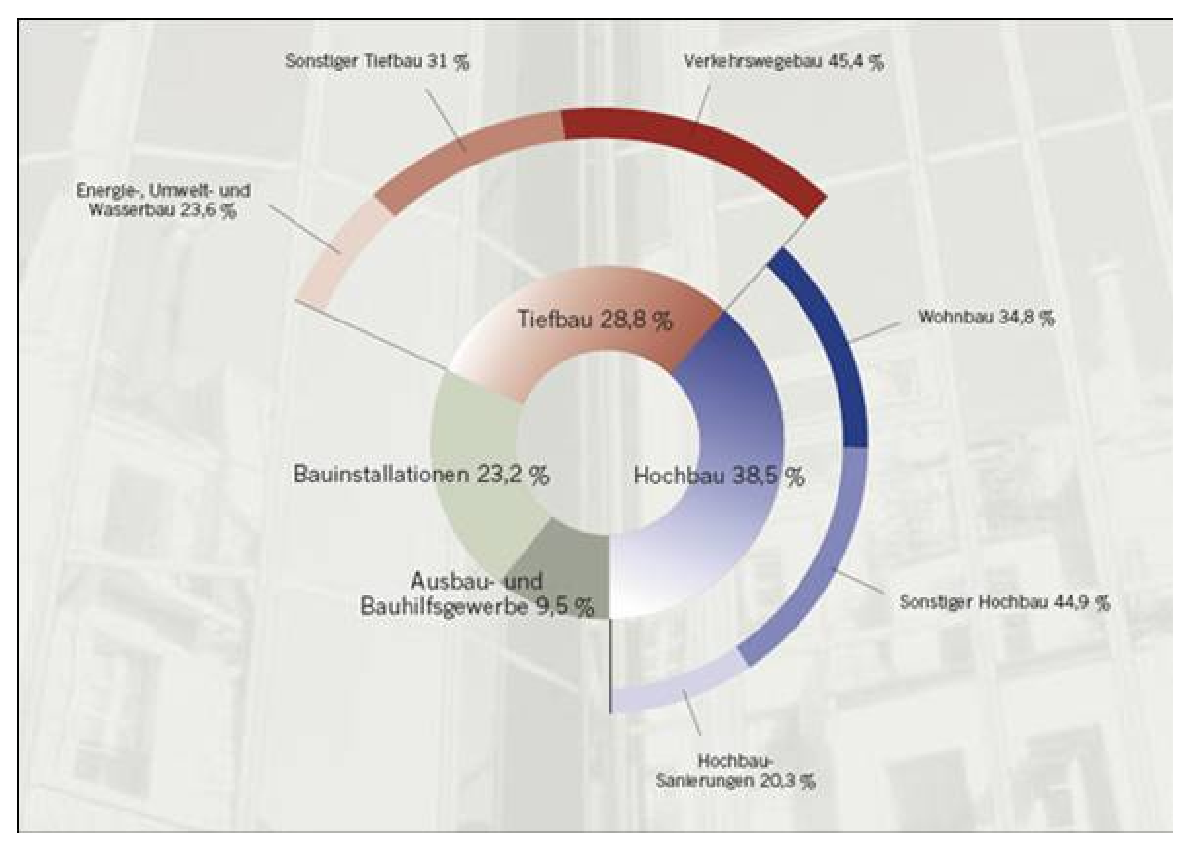
\includegraphics[width = 0.7\textwidth]{branche.eps}

\subsubsection{Konjunktur}
\label{sec:Konjunktur}

\section{Branchenanalyse nach Porter}
\label{sec:Porter}

\subsection{Wettbewerb in der Branche}
\label{sec:Wettbewerb}

%\input{martin.tex}

\subsection{Potentielle Mitbewerber}
\label{sec:Mitbewerber}

%\input{matthias.tex}

\subsection{Substitute}
\label{sec:Substitute}

%\input{stefan.tex}

\subsection{Lieferanten}
\label{sec:Lieferanten}

%\input{geri1.tex}

\subsection{Kunden}
\label{sec:Kunden}

%\input{geri2.tex}

\section{Bewertung und Zukunftsbild}
\label{sec:Bewertung}

\section{Zusammenfassung}
\label{sec:Zusammenfassung}

hier eine Tabelle mit Zusammenfassung und Aussage, ob weiter investiert werden soll!!!



\appendix

\section{erster Anhang}

%
\includegraphics[width = 0.7\textwidth]{logo.eps}


\end{document}
